\section{\label{intro}Introduction}

Nowadays, visual impairment remains at the heart of important social challenges. About 253 million people worldwide suffer from vision loss, with 36 million affected by a complete and irreversible blindness \citep{ref1}. Ocular pathologies are the main cause of visual impairment globally, as they generally lead to a loss of sight and can deteriorate to total blindness in some cases \citep{Foster}.
Chronic eye diseases are numerous \citep{ref4}, but recent studies show that moderate to severe visual impairment and blindness are often generated by four main ocular pathologies: cataracts, age-related macular degeneration, diabetic retinopathy, and glaucoma \citep{ref5,ref2}. 

Glaucoma is a neurodegenerative eye disease, which alters the optic nerve head (ONH) \citep{ref3}. This neuropathy is highlighted by a progressive lack of vision sensitivity, potentially leading to blindness at term. The early stage of glaucoma does not generate symptoms or changes to the visual field \citep{ref15}. However, as the disease develops, a gradual narrowing of visual field occurs, starting from the periphery and extending towards the center. If glaucoma is not treated, the disease can lead to complete blindness \citep{ophthal1}. 

This paper deals with efficient early glaucoma screening and diagnosis, to ensure regular and more accessible eye tests. It is important to have early treatment to help stop the vision becoming severely affected. Glaucoma is known as affecting a significant part of the population worldwide, with more than 64 million cases reported in 2013 globally, and estimations reaching 80 million and 111.8 million cases respectively by 2020 and 2040 \citep{ref3,ref11}.
Although the presence of the disease is generally influenced by factors such as aging or ethnicity, glaucoma is unfortunately present for any age group or population type, and both developed and developing countries are targeted \citep{Kingman}.
Glaucoma is also responsible for blindness in approximately 4.5 million people from all countries, making the neuropathy the second main cause of complete vision loss worldwide (12\% of the total burden population) \citep{ref11}. 
Moreover, due to its asymptomatic feature at the early stage, 70 to 90\% of the subjects suffering from glaucoma worldwide are unaware of the presence of the disease \citep{ref13,ref12}.
Because glaucoma develops in silence, yields irreversible damages to vision, and for all of the reasons exposed above, it is critical to provide early screening and diagnosis.
Then, this allows a more successful disease follow-up, in combination with a treatment able to slow down the spreading disease \citep{ref15,ref14}.

\begin{figure}[t]
    \centering
    
    \begin{tabular}{c c c c}
    {} & (a) & {} & (b) \\
    (1) & 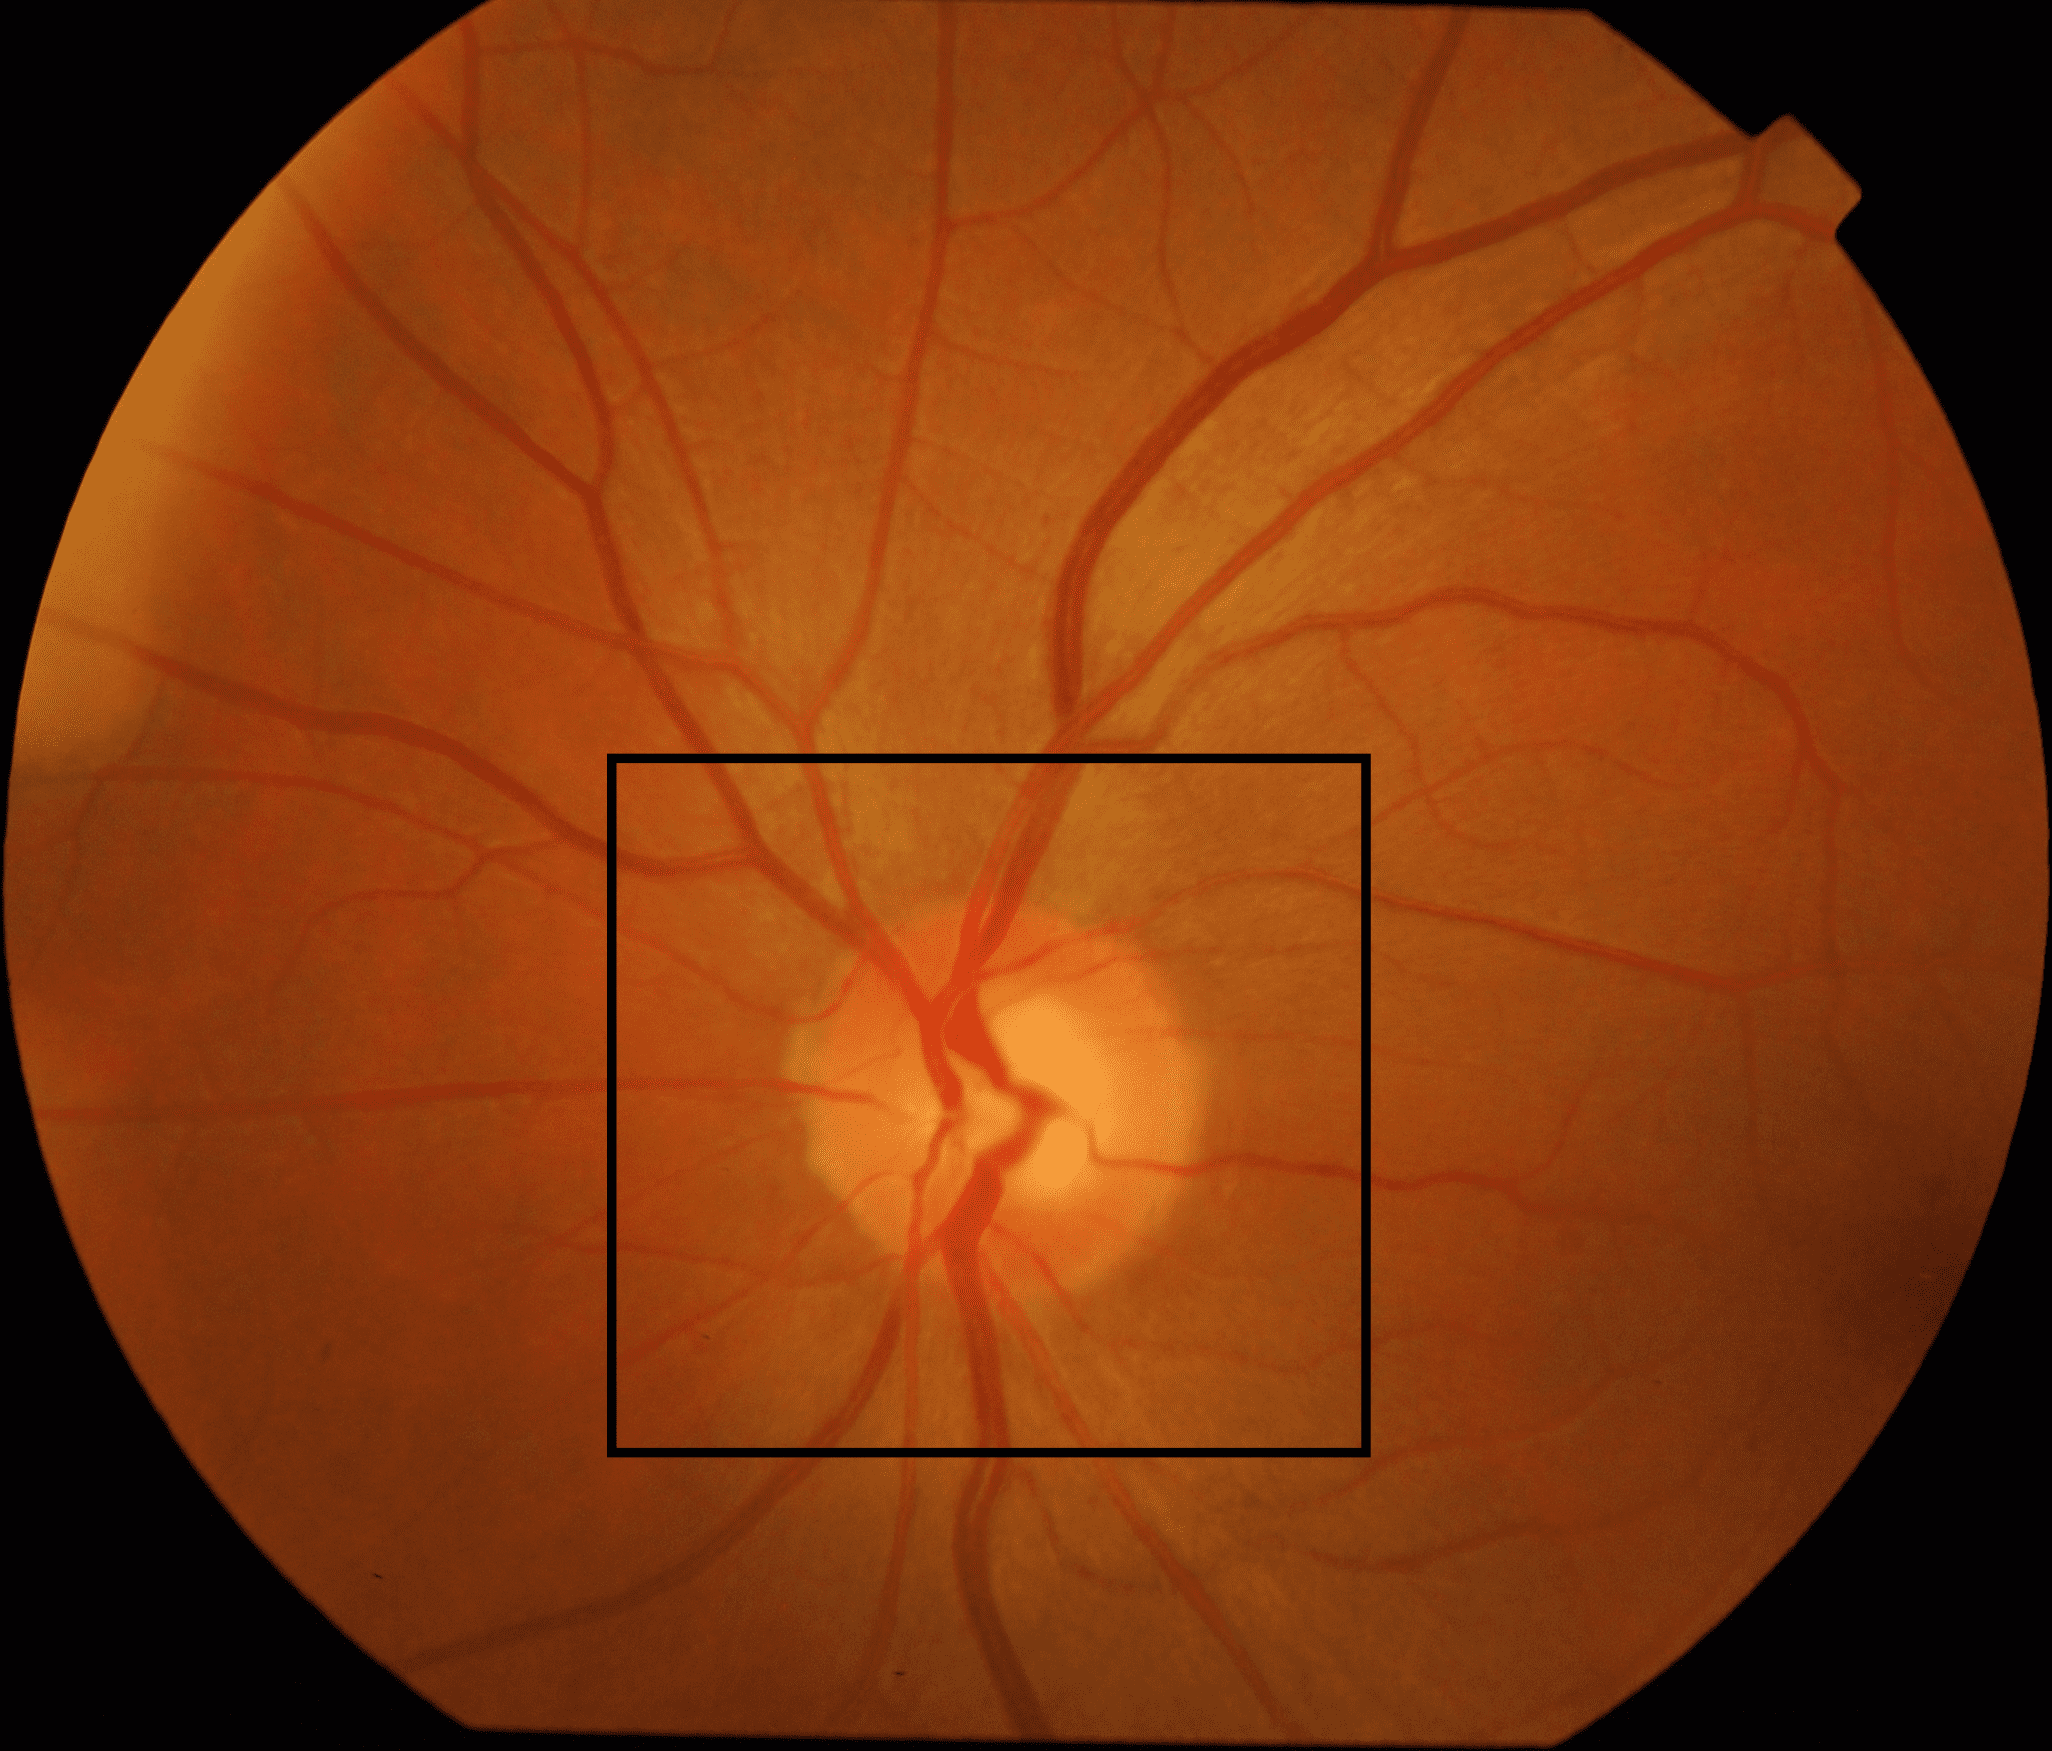
\includegraphics[height=3.0cm]{Images/Introduction/image1.png} & {} & 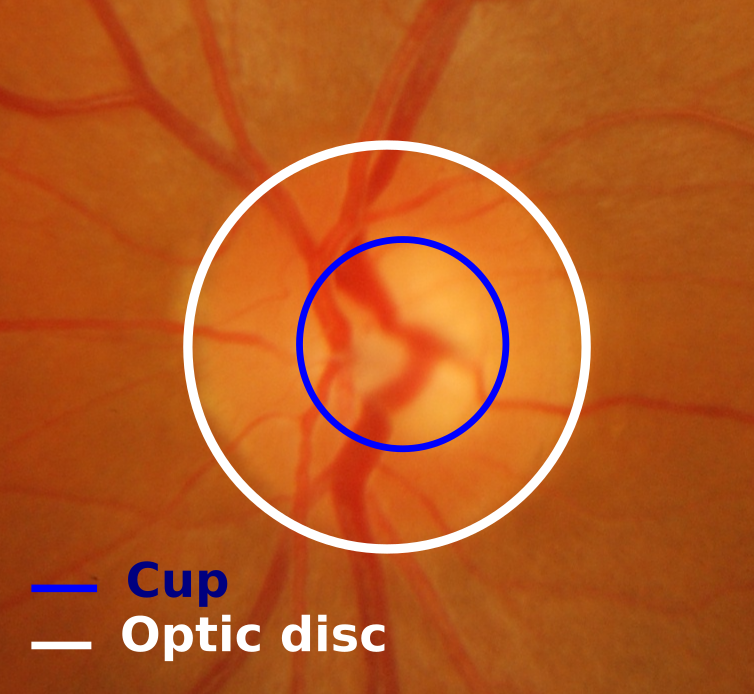
\includegraphics[height=3.0cm]{Images/Introduction/image1_zones.png} \\
    
    (2) & 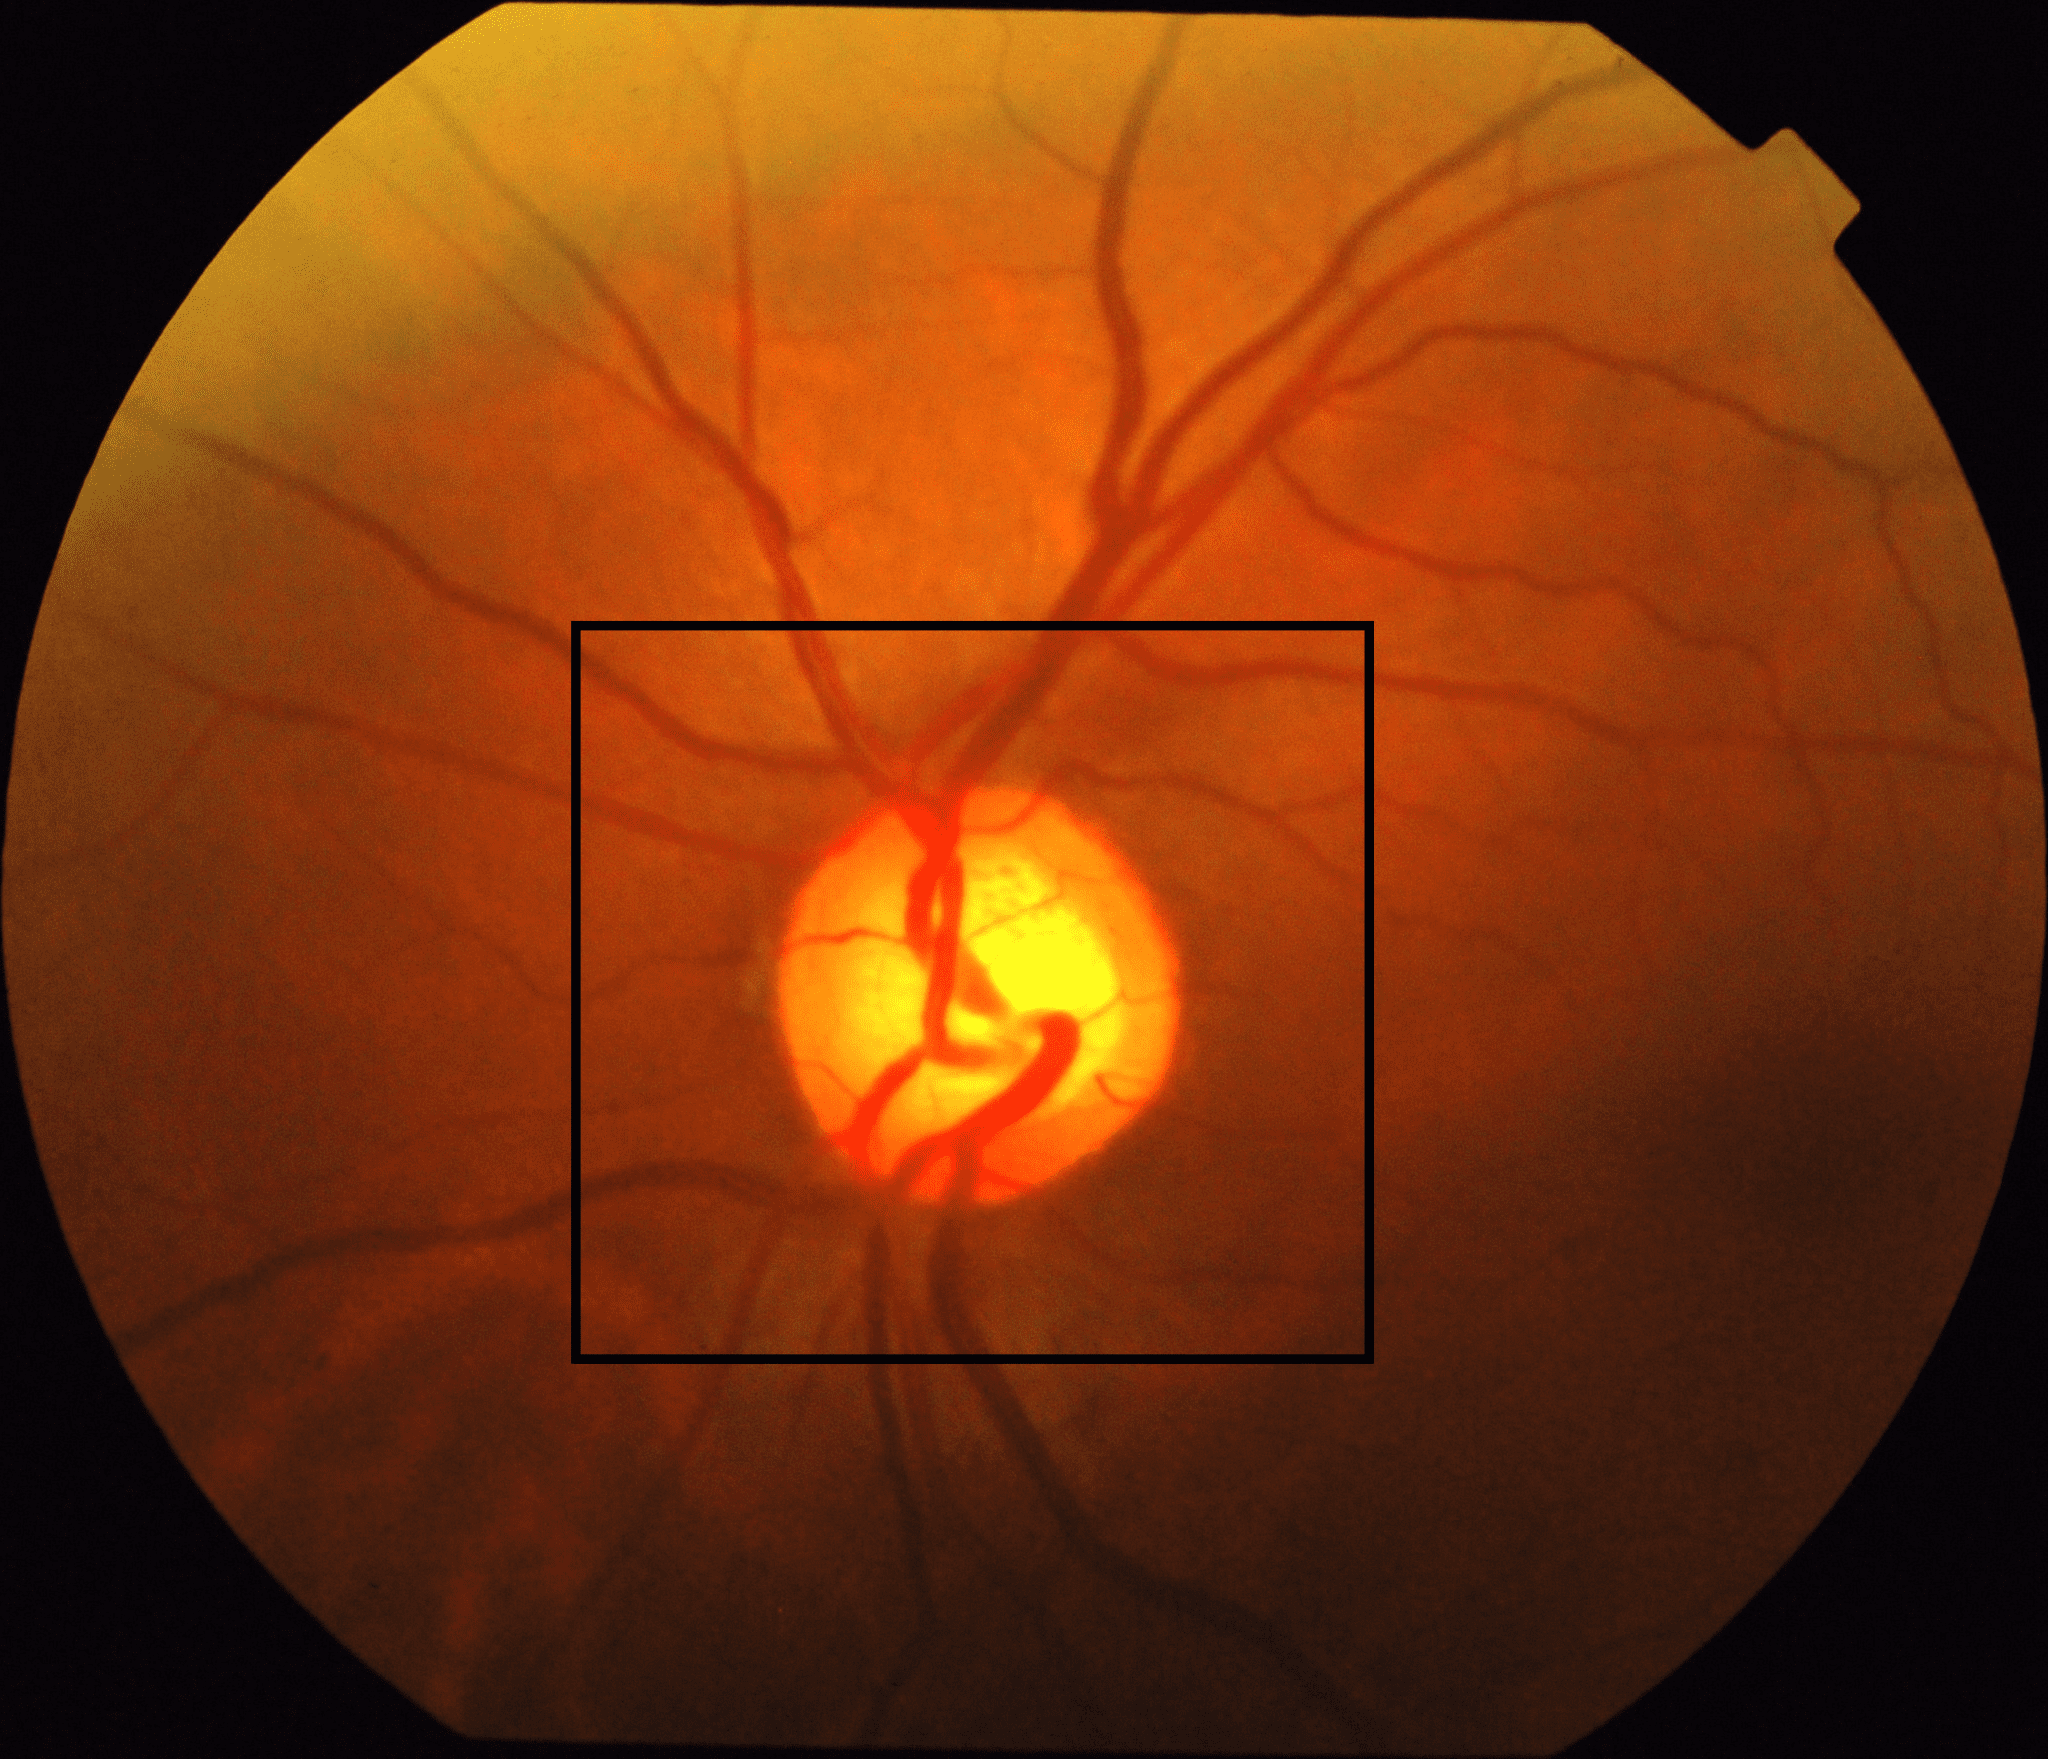
\includegraphics[height=3.0cm]{Images/Introduction/image2} & {} & 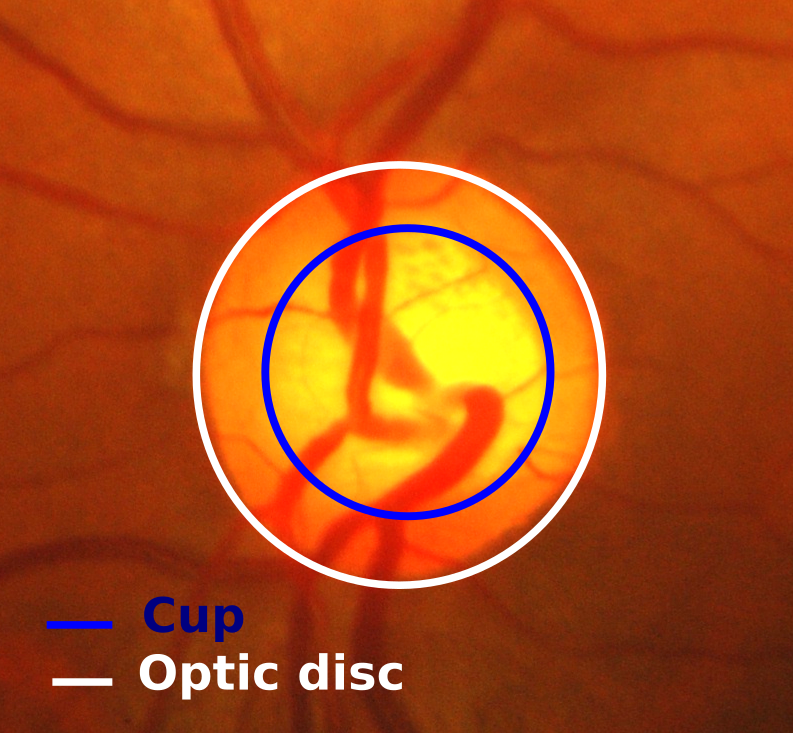
\includegraphics[height=3.0cm]{Images/Introduction/image2_zones.png} \\
    \end{tabular}

    \caption{Example of healthy (1) and glaucomatous (2) retinal images: (a) Retinal image with framed optic disc (OD) region, (b) OD sub-image with OC and OD areas.}
    \label{Example}
    
\end{figure}


In addition to visual field variation, two main tests allow glaucoma detection. The first consists in measuring the intraocular pressure (IOP) with a tonometer, and rating an abnormal high pressure rate. However, IOP measurement is not always a reliable and sufficient criterion for glaucoma assessment, as the presence of the disease does not necessarily induce an increase in IOP \citep{centreeyeres}.
The second is the assessment of the optic nerve head (ONH), the region in the retina where blood vessels converge and through which visual information transits to the brain. The ONH is composed of a bright circular region called the optic disc (OD), and inside the OD, a brighter region called the optic cup (OC) is apparent.
In \mbox{Fig. \ref{Example}}, two retinal images are presented, showing a sub-window around the ONH, with each of the OD and OC borders. Glaucoma goes with ONH appearance changes, as the OC region becomes more prominent as shown with both healthy (1) and glaucomatous (2) cases.

The evaluation of the changes in ONH appearance could generally be operated in two ways. The specialist examination is the most common way for ONH assessment, nevertheless, it suffers from subjectivity, time-consuming and significant costs \citep{liu}. Manual assessment can also be unpleasant for the patient \citep{ophthal1}.
The second way is more promising and efficient for glaucoma screening, and consists in a retinal image study \citep{abramoff}. Many works have been conducted in this direction, offering more accuracy on the final diagnosis, less workload for the specialist, and useful mass screening programs. 

Detecting the presence of the disease from retinal images consists in assessing the ONH and the retinal nerve fiber layer (RNFL), by extracting indicators such as the Cup-to-Disc Ratio (CDR) \citep{cdr}, the Inferior Superior Nasal Temporal (ISNT) rule \citep{isnt}, the RNFL thickness \citep{medeiros}, parapapillary atrophy \citep{Jonas} or ONH hemorrhagies \cite{fingeret}. When the other indicators are difficult to quantify without 3D-OCT imaging, the CDR appears as a relevant clinical feature for the assessment of ONH structural changes, as well as for detecting referable glaucomatous optic neuropathy from color fundus images \citep{foster2002definition, cheng}. Hence, exploiting the CDR contributes to the development of screening systems with 2-D dedicated snapshot devices and mobile platforms.

To implement CDR calculation for glaucoma screening, preliminary stages such as ONH detection, and both OC and OD areas segmentation are required \citep{singh2}. However, as this medical framework requires the fulfillment of specific constraints, performing these stages is difficult. In particular, facing a huge variety of clinical cases is a challenging task, when non-robust OD detection or inaccurate OC and OD segmentation are ongoing issues \citep{cheng}. Hence, in this disease screening context, overcoming limitations of existing methods at these respective stages is momentous.

Since early glaucoma diagnosis is primordial due to the irreversible vision damages caused during its progression, and to fill in the gaps of state-of-the-art screening methods, this paper proposes a new fully-automatic method for early glaucoma screening and diagnosis. Using 2-D retinal images, our proposed method calculates the CDR to carry out the final diagnosis. Our contributions are: an efficient OD detection method, a new OC and OD segmentation method, CDR calculation and glaucoma screening. These contributions form part of a mobile computer-aided system for automatic screening of eye diseases we are developing \citep{elloumi}.
Hence, in parallel of the proposed method, a rigorous synthesis of its computational efficiency is made. The complete methodology allows an effective and reliable diagnosis-help system, which can be part of useful screening programs developing the universal access to the eye health \citep{blanckenberg,bourouis}. 

The remainder of this paper is organised as follows. \mbox{Section \ref{related_work}} presents an overview of the CDR-based state-of-the-art works for glaucoma screening and diagnosis. In \mbox{section \ref{proposed_method}}, the proposed method is explained. In \mbox{section \ref{materials_results}}, materials are described and experimental results are shown. \mbox{Section \ref{discussion}} discuss about the proposed methodology. Finally, the conclusion and perspectives appear in \mbox{section \ref{conclusion_perspectives}}.

%Starting from the retinal image acquisition, we deliver the final glaucoma diagnosis.